\chapter{روش ارائه شده در پژوهش}
%\thispagestyle{empty}

\section{مقدمه}
در فصل‌های گذشته، سیر پژوهش‌‌های مرتبط در حوزه تولید خودکار شرح بر تصاویر را مورد بررسی قرار دادیم. در حال حاضر، تمامی پژوهش‌های انجام شده در حوزه تولید خودکار شرح بر تصاویر، با استفاده از شبکه‌های عصبی و یادگیری عمیق و با بهره‌گیری از چارچوب کاری رمزگذار-رمزگشا انجام می‌شوند. در پژوهش جاری، ما نیز از همین رویکرد استفاده می‌نماییم. 
\\
در این فصل، ابتدا به بیان چارچوب کاری رمزگذار-رمزگشای مورد استفاده در پژوهش، پرداخته و سپس مشکلات موجود در این چارجوب کاری را بیان می‌نماییم. سپس در ادامه، به ارائه روش پیشنهادی برای حل این مشکلات و بررسی جوانب مختلف آن می‌پردازیم.

\section{رمزگذار}
رمزگذار مورد استفاده در چارچوب کاری رمزگذار-رمزگشا در حوزه تولید خودکار شرح بر تصاویر، یک شبکه عصبی کانولوشنی عمیق است که به‌ ازای هر تصویر ورودی،‌ یک بردار ویژگی تولید می‌نماید. در پژوهش‌های مختلف، از شبکه‌های عصبی کانولوشنی مختلفی به این منظور استفاده می‌شود. عموما استفاده از این شبکه‌ها به طور از پیش آموزش دیده، اتفاق می‌افتد. در این حالت، شبکه‌های عصبی کانولوشنی را ابتدا روی یک مجموعه‌داده معتبر، که معمولا مجموعه داده \lr{ImageNet} است، آموزش می‌دهند. سپس از شبکه آموزش دیده، برای استخراج ویژگی از تصاویر، استفاده می‌نمایند. در پژوهش جاری، ما نیز از مدل \lr{Google Inception V3} که در پژوهش \cite{szegedy2016rethinking} توسط سِگِدی و همکارانش در سال 2016 ارائه شده است، به عنوان رمزگذار استفاده کرده‌ایم.
\\
یکی از اساسی‌ترین تغییراتی که در این مدل نسبت به مدل‌های گذشته خود ارائه شده است، جایگزینی فیلترهای کانولوشن $5*5$ با یک شبکه عصبی کوچک با دو فیلتر $3*3$ است. شکل \ref{fig:conv53} نمونه‌ای از این شبکه عصبی را نمایش می‌دهد. همان‌طور که در شکل مشخص است، عملی که این شبکه عصبی کوچک انجام می‌دهد، دقیقا معادل عملیاتی است که کانوالو کردن یک فیلتر $5*5$ روی یک تصویر انجام می‌دهد. این جایگزینی با کاهش تعداد پارامترهای مورد نیاز، سرعت یادگیری و عمل‌کرد شبکه را بهبود می‌بخشد. 
\begin{figure}[h]
	\centering
	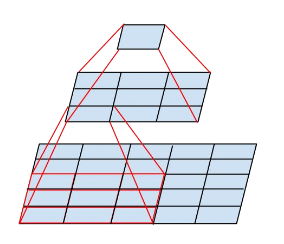
\includegraphics[scale=0.5]{Imgs/inceptionConv53.png}
	\caption[شبکه عصبی کوچک جایگزین فیلتر $5*5$]{شبکه‌ عصبی کوچک جایگزین فیلتر $5*5$ ارائه شده در پژوهش \cite{szegedy2016rethinking}}
	\label{fig:conv53}
\end{figure}
\\
به همین ترتیب می‌توان فیلتر‌های $n*n$‌ را به فیلتر‌های $1*n$ و $n*1$ تبدیل کرد. این کار، می‌تواند بهبود قابل ملاحظه‌ای در عمل‌کرد شبکه ایجاد نماید.
\\
ساختار کلی رمزگذار مورد استفاده در این پژوهش، در شکل \ref{fig:encoder} ارائه شده است. همان‌طور که در این شکل قابل مشاهده است، ورودی‌های این شبکه، تصاویر رنگی به ابعاد 299 در 299 پیکسل هستند. با توجه به این‌که تصاویر موجود در مجموعه‌داده مورد استفاده در این پژوهش، محدودیت ابعاد ندارند، ابعاد تمام تصاویر را به اندازه‌ای کاهش می‌دهیم که در یک قاب 299*299 پیکسل، جای بگیرند. سپس قسمت‌های اضافی قاب را با پیکسل‌های صفر می‌پوشانیم و تصویر آماده شده را به شبکه می‌دهیم.

\begin{figure}[h]
	\centering
	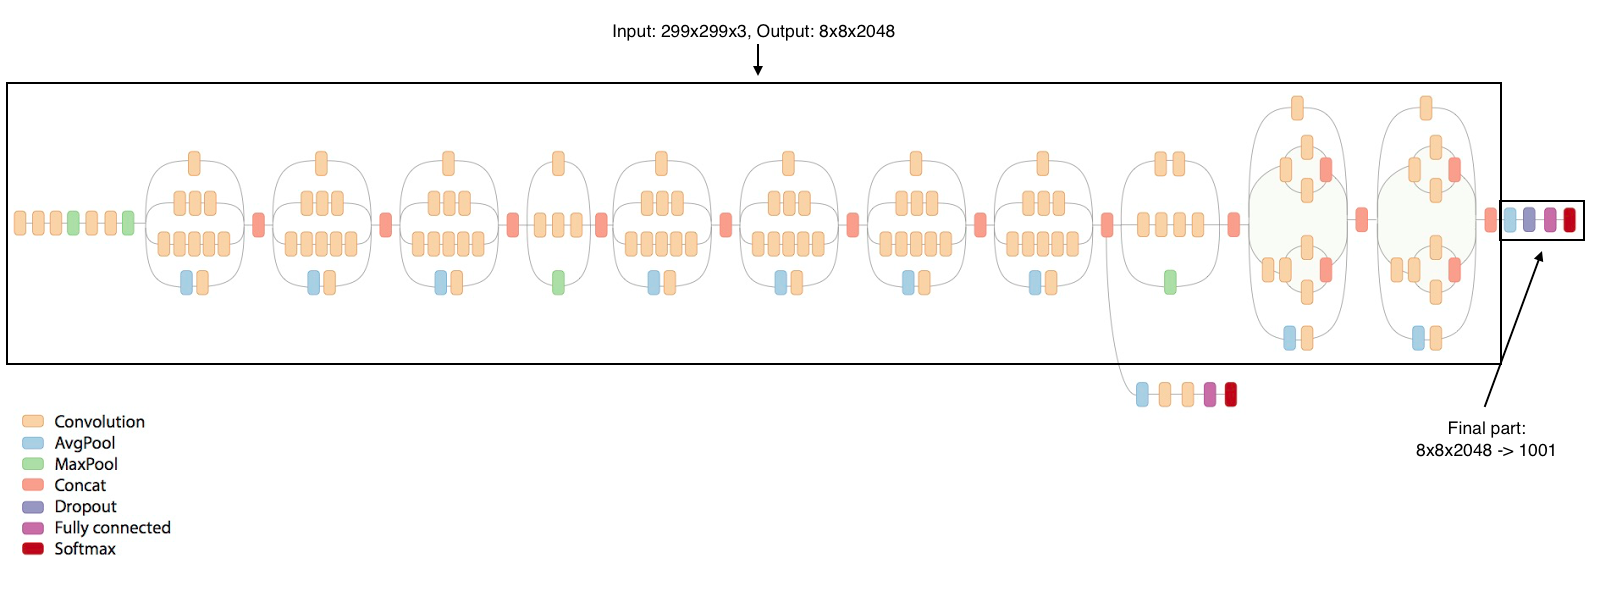
\includegraphics[scale=0.25]{Imgs/encoder.png}
	\caption[ساختار کلی رمزگذار مورد استفاده در پژوهش]{ساختار کلی رمزگذار مورد استفاده در پژوهش \cite{szegedy2016rethinking}}
	\label{fig:encoder}
\end{figure}

همان‌طور که در شکل \ref{fig:encoder} قابل مشاهده است، بخش پایانی رمز‌گذار شامل لایه‌هایی است که $8*8$ بردار ویژگی $2048$ بعدی را گرفته، بردارهای ویژگی مورد استفاده برای انتقال یادگیری\enfootnote{Transfer Learning}، و یک بردار ویژگی نهایی 1008 بعدی را خروجی می‌دهد. بردار ویژگی حاصل، با اعمال یک لایه تماماً متصل\enfootnote{Fully Connected Layer} روی خروجی، تولید شده است. این لایه به منظور آموزش شبکه عصبی برای دسته‌بندی اجسام موجود در تصاویر، ایجاد شده است. 
\\
از آن‌جا که دسته‌بندی اجسام، برای تولید خودکار شرح بر تصاویر، به تنهایی کافی نیست، در این پژوهش به جای استفاده از بردار ویژگی لایه آخر، از $8*8$ بردار ویژگی 2048 بعدی مربوط به انتقال یادگیری، استفاده می‌نماییم. هر کدام از این بردارهای ویژگی استخراج شده، بیان‌کننده اطلاعات کل تصویر است. با این‌ حال، تمرکز هر یک از این بردارها به بخشی از تصویر اولیه معطوف شده است. با این تفاسیر،‌ این بردارها می‌توانند به عنوان بردارهای حاشیه‌نویسی مناسب مورد استفاده قرار بگیرند. 
\\
با توجه به این نکته که، مدل از پیش آموزش دیده این شبکه عصبی، که روی مجموعه‌داده \lr{ImageNet} آموزش داده شده است، در دسترس و قابل استفاده برای پژوهش‌گران دیگر است و نتایج اعمال این مدل بر مجموعه‌داده مذکور، بهتر از تمامی مدل‌های قبلی ارائه شده برای دسته‌بندی تصاویر بوده است، در پژوهش حاضر، از نسخه در دسترس این شبکه، بدون آموزش مجدد برای تولید خودکار شرح بر تصاویر به ترتیبی که توضیح داده شد، استفاده می‌شود. جدول \ref{tbl:encoder} نتایج حاصل از این شبکه عصبی را با بهترین نتایج حاصل‌ از روش‌های قبلی مورد مقایسه قرار داده است.

\begin{table}[h]
	\centering
	\caption{مقایسه عمل‌کرد رمزگذار مورد استفاده در پژوهش با مدل‌های دیگر\cite{szegedy2016rethinking}}
	\label{tbl:encoder}
	\begin{tabular}{|c|c|c|}
		\hline
نام روش
		‌&
		 خطای محتمل‌ترین دسته
		\enfootnote{Top-1 Error}
		& 
		خطای ۵ محتمل‌ترین دسته
		\enfootnote{Top-5 Error}
		\\
		\hline
		\lr{GoogLeNet}\cite{szegedy2015going} & - & 6.67\%
		\\
		\lr{PReLU}\cite{he2015delving} & 20.1\% & ‌4.9\%
		\\
		\lr{Inception-V3} & 17.2\% & 3.58\%
		\\
		\hline
	\end{tabular}
\end{table}



\section{رمزگشا}
در این بخش به بررسی مدل ارائه شده به عنوان رمزگشا و فرایند پیشنهادی تولید جمله می‌پردازیم. در ادامه این قسمت از گزارش، ابتدا مدل استاندارد رمزگشا را مورد بررسی قرار می‌دهیم. سپس با بیان ایده اصلی پژوهش در ارتقا کیفیت جملات تولید شده و بررسی جزئیات آن، نحوه تغییر ساختار رمزگشا، تابع هزینه و متد آموزش را بررسی خواهیم نمود.
\subsection{معماری رمزگشا}
وظیفه واحد رمزگشا در چارچوب کاری رمزگذار-رمزگشا این است که با دریافت بردارهای حاشیه‌نویسی تصویر، جملات توصیف‌کننده مربوط به تصویر را تولید نماید. هر جمله را می‌توان به عنوان دنباله‌ای با طول متغیر از کلمات در نظر گرفت که هر کلمه در آن، با یک بردار ویژگی توصیف شده است. رابطه \eqref{eq:X} نمایش یک جمله در مدل ریاضی مورد استفاده در این پژوهش را بیان می‌کند که در آن، $L$ تعداد کلمات موجود در جمله و $x_i$ بردار ویژگی کلمه $i$ام در جمله است. لازم به ذکر است، در ادامه این بخش، جملات و کلمات ورودی رمزگشا را با $X$‌ و جملات و کلمات خروجی را با $Y$ نمایش می‌دهیم.

\begin{equation}
	X = \{x_1, x_2, \cdots, x_L\}
	\label{eq:X}
\end{equation}

فرایند یادگیری رمزگشا، باید به نحوی انجام شود که رمزگشا بتواند شرح متناظر هر تصویر را برای تصاویر و شرح موجود در مجموعه‌داده‌ آموزشی، تولید نماید. برای این منظور، با فرض این‌که بردارهای حاشیه‌نویسی استخراج شده توسط رمزگذار برای تصویر $I$ با $\Theta = \{\theta_0, \cdots, \theta_n\}$  و جمله مطلوب در مجموعه‌داده برای تصویر $I$ را با 
$S = \{s_1, \cdots, s_{L_I}\}$
 نمایش داده شده باشند، رمزگشا باید بتواند در هر مرحله، احتمال کلمه بعدی را با توجه به کلمات تولید شده قبلی و مجموعه بردارهای حاشیه‌نویسی تولید نماید. به این منظور، باید یک مساله بهینه‌سازی را تعریف نموده و درصدد حل آن باشیم. رابطه \eqref{eq:obj1} مساله بهینه‌سازی اولیه‌ای را نمایش می‌دهد که با حل آن می‌توان رمزگشای مورد نظر را تولید کرد. در این رابطه $\Xi$ مجموعه‌ تمام متغیرهای قابل آموزش است. 
\begin{align*}
	\underset{\Xi}{maximize} \>\> &Pr(y_{t+1} | y_t, y_{t-1}, \cdots, y_0, \Theta) \\
	s.t. \>\>\>\>\> &y_{t+1} = s_{t+1}
	\numberthis
	\label{eq:obj1}
\end{align*}

مطابق با مساله بهینه‌سازی تعریف شده، به دنبال مدلی هستیم که در هر مرحله بتواند یک تابع احتمال روی تمام کلمات موجود در دیکشنری کلمات ایجاد نماید. این تابع احتمال، یک تابع احتمال شرطی، به شرط داشتن کلمات تولید شده قبلی و مجموعه بردارهای حاشیه‌نویسی استخراج شده توسط رمزگذار است. در این تابع احتمال باید تا جای ممکن، احتمال کلمه بعدی موجود در شرح متناظر تصویر، زیاد و احتمال بقیه کلمات، کم باشد. پس باید تمام پارامترهای قابل آموزش را طوری مقداردهی نماییم، که کلمه $t+1$ در شرح متناظر تصویر، بیشترین احتمال را بین کلمات دیکشنری در مرحله $t$ام داشته باشد.
\\

واحد اساسی سازنده رمز‌گشای مورد استفاده در این پژوهش، شبکه عصبی \lstm است. روابط \eqref{eq:lstm1} تا \eqref{eq:lstm5}، ساختار داخلی یک واحد \lstm را نمایش میدهد. در این روابط، $x$ بردار ورودی، $h$ بردار حالت شبکه، $f$ گیت فراموشی، $i$ بردار فعالیت ورودی، $o$ بردار خروجی، $c$ بردار وضعیت سلول و $t$ اندیس زمان هستند. همین‌طور $\sigma_g$‌ تابع سیگموئید و $\sigma_c$ تابع تانژانت هایپربولیک را نمایش می‌دهند. به علاوه، بردارهای $W$ و $U$ به ترتیب بردارهای وزن ورودی و حالت شبکه و بردارهای $b$‌ بردارهای بایاس هستند. نماد $\odot$ بیان‌گر ضرب مولفه‌های نظیر به نظیر، ضرب هادامارد\enfootnote{Hadamard Multiplication}، است. 

\begin{align*}
	f_t &= \sigma_g(W_fx_t + U_fh_{t-1} + b_f)
	\numberthis
	\label{eq:lstm1}
	\\
	i_t &= \sigma_g(W_ix_t + U_ih_{t-1} + b_i)
	\numberthis
	\label{eq:lstm2}	
	\\
	o_t &= \sigma_g(W_ox_t + U_oh_{t-1} + b_o)
	\numberthis
	\label{eq:lstm3}	
	\\
	c_t &= f_t \odot c_{t-1} + i_t \odot \sigma_c(W_cx_t + U_c h_{t-1} + b_c) 
	\numberthis
	\label{eq:lstm4}
	\\
	h_t &= o_t \odot c_t
	\numberthis
	\label{eq:lstm5}		
\end{align*}

شکل \ref{fig:lstm}، نمایی از یک سلول شبکه \lstm را نمایش می‌دهد. در پروژه حاضر، از این ساختار به عنوان واحدهای اصلی شبکه رمزگشا استفاده می‌نماییم. 

\begin{figure}[h]
	\centering
	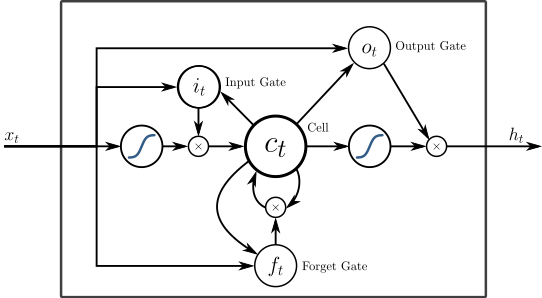
\includegraphics[scale=0.5]{Imgs/lstm.png}
	\caption{نمایی از یک سلول شبکه \lstm}
	\label{fig:lstm}
\end{figure}


به منظور افزایش قدرت شبکه، واحدهای \lstm را به صورت‌ پشته‌ای روی هم چیده و از مجموعه واحد‌های موجود در یک پشته، به عنوان یک واحد عملیاتی در یک مرحله زمانی استفاده می‌نماییم. شکل \ref{fig:stackedLstm} طرح‌واره‌ای از ساختار رمزگشای پشته‌ای را نمایش می‌دهد.

\begin{figure}[h]
	\centering
	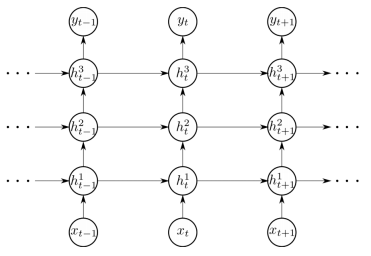
\includegraphics[scale=0.7]{Imgs/stackedLstm.png}
	\caption{طرح‌واره‌ای از ساختار \lstm پشته‌ای}
	\label{fig:stackedLstm}
\end{figure}

نکته قابل توجه این است که بردارهای تولیدی $y_t$ در این ساختار، همگی یک توزیع احتمال روی لغات دیکشنری را نمایش می‌دهند. اگر دیکشنری شامل تمام کلمات موجود در همه توصیفات موجود در مجموعه‌داده، شامل $\Gamma$ لغت باشد، همه بردارهای $y_t$ دارای $\Gamma$‌ مولفه هستند که هر مولفه $i$ از آن، احتمال رخ‌داد کلمه $i$ام در دیکشنری را در محل $t$ام از جمله ورودی مشخص می‌کند.
\\
برای تولید جملات، کافیست در هر مرحله، با توجه به توزیع احتمال مشخص‌ شده توسط بردار خروجی شبکه در همان مرحله،‌ یک کلمه را از دیکشنری کلمات استخراج نموده و در جمله قرار دهیم.
\\

\subsubsection{ارائه ایده اصلی برای بهبود روش}
مطابق با معماری استاندارد مورد استفاده برای رمزگشا در چارچوب کاری رمزگذار-رمزگشا و با توجه به مساله بهینه‌سازی \eqref{eq:obj1} خروجی شبکه بردار توزیع احتمال روی تمام کلمات دیکشنری در هر مرحله است. خطای مدل در زمان آموزش با مقایسه بردار خروجی شبکه و بردار مطلوب، که با توجه به شرح مربوط به تصویر در مجموعه‌داده ایجاد شده است، محاسبه می‌شود. این بردار مطلوب به صورت تک‌فعال\enfootnote{One Hot Vector} تولید می‌شود؛ به این معنی که برای تولید بردار مطلوب در مرحله $t$ام، کلمه $t$ام موجود در شرح تصویر را انتخاب کرده، اندیس آن کلمه را در دیکشنری کلمات پیدا می‌نماییم. سپس یک بردار صفر به طول $\Gamma$ ایجاد نموده و مولفه‌ای را که اندیس آن در بردار، با اندیس کلمه در دیکشنری برابر است، با عدد یک مقداردهی می‌نماییم.
\\
در این مدل آموزش، شبکه سعی در یادگیری تولید دقیق جملات موجود می‌نماید و از آن‌جا که استفاده از معانی کلمات در هیچ‌جایی از این فرایند دیده نشده است، قراردادن کلمات هم‌معنی به جای یک‌دیگر در جملات تولید شده، که باعث ایجاد جملات گوناگون و عمل‌کرد بهتر شبکه می‌شود، در این مدل، امکان‌پذیر نیست.
\\
علاوه بر مورد فوق، با مدل‌سازی توزیع احتمال روی تمام دیکشنری، ابعاد مورد انتظار در خروجی شبکه بسیار زیاد شده و تعداد پارامترهای قابل آموزش، به بیش از 100 میلیون پارامتر می‌رسد. تعداد زیاد پارامترهای قابل آموزش، یادگیری شبکه را دچار مشکل کرده و علاوه بر افزایش زمان یادگیری و استفاده از شبکه، باعث حساسیت بیشتر مدل به فوق‌پارامترهای\enfootnote{Hyperparameters} الگوریتم‌های یادگیری، مانند نرخ یادگیری،‌ می‌شود.
\\
در این پژوهش، مدل‌سازی جاسازی کلمات به جای مدل توزیع احتمال آن‌ها، برای بهبود معماری فعلی، پیشنهاد می‌شود. معماری فوق را می‌توان به گونه‌ای تغییر داد که شبکه به جای مدل‌سازی توزیع احتمال شرطی کلمات،‌ جاسازی آن‌ها را مدل نماید. جاسازی کلمات در ابعاد به مراتب کم‌تری از ابعاد دیکشنری قابل انجام است. با جای‌گزینی بردار جاسازی به جای بردار تک‌فعال کلمات، ابعاد خروجی کاهش یافته و پیرو آن، تعداد پارامترهای قابل آموزش شبکه به شکل چشم‌گیری کاهش پیدا می‌کنند. کاهش تعداد پارامترهای قابل آموزش به طور مستقیم، سرعت یادگیری را افزایش داده و از استفاده از بردارهای تنک در فرایند آموزش،‌ جلوگیری می‌نماید.
\\
بردار جاسازی کلمات، نماینده معنای کلمات است. استفاده از بردار جاسازی کلمات در لایه خروجی، علاوه بر مزایای فوق، شبکه را قادر می‌سازد تا از اطلاعات معنایی لغات استفاده کرده و بتواند کلمات هم‌معنی با کلمات موجود در مجموعه‌داده را نیز به جای آن‌ها در جملات قرار دهد. این کار علاوه بر سهولت در یادگیری شبکه، امکان ایجاد جملات جدید را بیشتر کرده و عمل‌کرد شبکه در تولید جمله را بهبود می‌بخشد.
\\
به منظور جایگزینی جاسازی کلمات به جای بردار تک‌فعال، باید اولا مساله بهینه‌سازی مطرح را تغییر داده و سپس روش مناسب برای بهینه‌سازی را انتخاب نماییم. علاوه بر این، لازم است، مدلی برای تولید جاسازی مناسب برای کلمات ایجاد کرده و آن را به مدل فعلی اضافه نماییم. در ادامه به بررسی جزئیات مربوطه می‌پردازیم.
\subsection{جاسازی کلمات}
مدل جاسازی استفاده شده در این پژوهش، مطابق با مدل ارائه شده در پژوهش \cite{mikolov2013distributed} است که توسط آقای میکولوف و همکارانش در سال 2013 ارائه شده است. ویژگی برجسته این پژوهش این است که از مدل \lr{Skip-Gram}، که در پژوهش \cite{mikolov2013efficient} ارائه شده است، استفاده می‌نماید.
\\
نکته مطلوب در مدل \lr{Skip-Gram} این است که بردار جاسازی مربوط به کلمات، طوری تعیین می‌شود که احتمال تشخیص صحیح کلمات پیرامون کلمه جاری، بیشینه شود. به عبارت بهتر، با داشتن کلمه جاری، به راحتی بتوان کلمات قبل و بعد از آن را مشخص نمود. رابطه \eqref{eq:embd} تابع هدف این مدل را نمایش می‌دهد. در این رابطه،‌ $x_t$ کلمه فعلی را نمایش می‌دهد. مدل مذکور به نحوی آموزش می‌بیند که بتواند رابطه \eqref{eq:embd} را بیشینه کند.
\begin{equation}
	\frac{1}{T} \Sigma_{t=1}^T \Sigma_{-c \le j \le c, j \ne 0} log Pr(x_{t+j} | x_t)
	\label{eq:embd}
\end{equation}
تابع احتمال شرطی به کار رفته در رابطه \eqref{eq:embd} مطابق با رابطه \eqref{eq:embdpr} تعریف می‌شود که در آن، $\nu_{x_o}$ و $\nu_{x_i}$ به ترتیب، بردارهای جاسازی $x_o$ و $x_i$‌ و $\Gamma$ تعداد کلمات موجود در دیکشنری هستند.
\begin{equation}
	Pr(x_o | x_i) = \frac{exp(\nu^T_{x_o} . \nu_{x_i})}{\Sigma_{w=0}^\Gamma exp(\nu^T_{x_w} . \nu_{x_i})}
	\label{eq:embdpr}
\end{equation}
شکل \ref{fig:embd} طرح‌واره‌ای از مدل \lr{Skip-Gram} را نمایش می‌دهد. همان‌طور که در این شکل مشخص است، در این مدل به نحوی بردارهای جاسازی برای کلمات تولید می‌شود که خطای تشخیص کلمات قبل و بعد از هر کلمه با داشتن بردار جاسازی آن کلمه، به کم‌ترین مقدار ممکن برسد.

\begin{figure}[h]
	\centering
	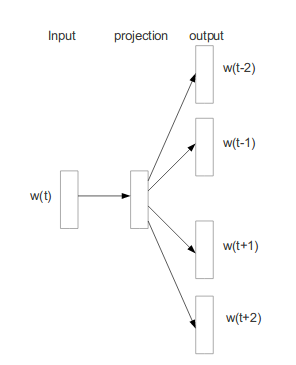
\includegraphics[scale=0.5]{Imgs/skipgram.png}
	\caption[طرح‌واره‌ای از مدل \lr{Skip-Gram}]{طرح‌واره‌ای از مدل \lr{Skip-Gram} ارائه شده در پژوهش \cite{mikolov2013distributed}}
	\label{fig:embd}
\end{figure}

با در نظر گرفتن این نکته که در این مدل، هدف اساسی در تولید بردارهای جاسازی، افزایش قابلیت تشخیص بردارهای جاسازی بعدی در جملات است، استفاده از این مدل جاسازی کلمات، علاوه بر مدل‌سازی معنای کلمه، فرایند یادگیری شبکه و تشخیص کلمات بعدی را بهبود می‌بخشد.
\\
در این پژوهش، ابتدا جاسازی کلمات با استفاده از مدل ارائه شده در پژوهش \cite{mikolov2013distributed} برای تمام کلمات موجود در مجموعه شرح‌های مجموعه‌آموزشی، محاسبه و ذخیره می‌شود. در تمام پژوهش، از همین بردارهای جاسازی به عنوان بردارهای ویژگی کلمات استفاده می‌شود.
\\
با تغییر مدل خروجی شبکه، از حالت بردار تک‌فعال، به بردار جاسازی به شرح فوق، مساله بهینه‌سازی قبلی نمی‌تواند منجر به یادگیری صحیح شبکه شود. در مدل جدید، به جای پیش‌بینی احتمال وقوع کلمات، باید یک مساله رگرسیون مناسب تعریف شود؛ به نحوی که خروجی شبکه در هر مرحله، هرچه بیشتر به بردار جاسازی کلمه مرحله بعدی، نزدیک شود. با این تفاسیر، مساله بهینه‌سازی \eqref{eq:obj1} به مساله بهینه‌سازی \eqref{eq:obj2} تبدیل می‌شود که در آن، $y_{t+1}$ خروجی شبکه در لایه آخر و $s_{t+1}$ بردار جاسازی کلمه $t+1$ام در جمله مربوط به تصویر ورودی است.

\begin{align*}
\underset{\Xi}{minimize} \>\> &tr\{E\{(y_{t+1}-s_{t+1})(y_{t+1}-s_{t+1})^T\}\}
\numberthis
\label{eq:obj2}
\end{align*}

در روش‌های قبلی، از آن‌جا که هدف اصلی، تولید توزیع احتمال کلمات در لایه آخر رمزگشا بود، از یک لایه \lr{Softmax} به منظور تبدیل خروجی شبکه به توزیع احتمال استفاده می‌شد. با توجه به تغییری که در این پژوهش انجام شد، نیازی به تولید توزیع احتمال در لایه آخر رمزگشا وجود ندارد و این لایه از معماری شبکه، حذف می‌شود.
\\
از طرف دیگر، استفاده از تابع هزینه \lr{Cross-Entropy}‌ به عنوان تابع خطای شبکه، در روش‌های قبلی مرسوم بود. رابطه \eqref{eq:cross}، نحوه محاسبه این تابع را برای توزیع‌های احتمال گسسته $p$ و $q$‌، مشخص می‌نماید. همان‌طور که در این رابطه مشخص است، این تابع هزینه، شباهت زیادی با معیار فاصله توزیع \lr{kullbak-leibler} دارد.
\begin{equation}
	H(p, q) = - \Sigma_x p(x) log (q(x))
	\label{eq:cross}
\end{equation}

این تابع هزینه، برای مدل‌سازی توزیع احتمال و آموزش شبکه برای پیش‌بینی یک توزیع احتمال در طول زمان، کارایی بسیار خوبی از خود نشان می‌دهد. اما از آن‌جا که مساله بهینه‌سازی شبکه رمزگشا در این پژوهش، با جای‌گزینی بردار جاسازی کلمات به جای بردار تک‌فعال، به مساله رگرسیون تغییر پیدا کرد، مطابق با مساله تعریف شده \eqref{eq:obj2}، از میانگین مربع خطا\enfootnote{Mean Squared Error} به عنوان تابع هزینه شبکه استفاده می‌نماییم. رابطه \eqref{eq:mse} نحوه محاسبه خطا را بیان می‌کند.
\begin{equation}
\epsilon = tr\{E\{(y_{t+1}-s_{t+1})(y_{t+1}-s_{t+1})^T\}\}
\label{eq:mse}
\end{equation}


\section{نحوه آموزش و تست شبکه}
در مرحله آموزش شبکه در این پژوهش از بهینه‌ساز آدام\enfootnote{Adam Optimizer}، که در پژوش \cite{kingma2014adam} توسط آقای کینگما و همکارانش در سال 2014 ارائه شد، استفاده شده است. بهینه‌ساز آدام، یکی از بهینه‌سازهای دسته نزول تصادفی در امتداد گرادیان
\enfootnote{Stochastic Gradient Descent}
 به شمار می‌رود. این بهینه‌ساز در مسائلی که فضای پارامترهای قابل آموزش آن‌ها بسیار بزرگ است، عمل‌کرد بسیار خوبی از خود نشان می‌دهد. استفاده از این بهینه‌ساز در بین پژوهش‌های مربوط به تولید خودکار شرح بر تصاویر و مدل‌سازی زبان طبیعی، رایج است.
\\
به منظور جلوگیری از بیش‌برازش\enfootnote{Overfitting} شبکه روی مجموعه‌داده آموزشی، از منظم‌سازی\enfootnote{Regularization} حذف نود\enfootnote{Drop Out} استفاده شده است. این منظم‌سازی روی تمام لایه‌های داخلی شبکه رمزگشا، اعمال شده است. در مواقعی که شبکه عصبی بازگشتی، خیلی بزرگ باشد و تعداد پارامترهای قابل آموزش آن زیاد باشند، استفاده از این منظم‌ساز باعث حذف برخی از واحدهای شبکه شده و از بیش‌برازش شبکه روی داده‌های مجموعه‌داده آموزشی، جلوگیری می‌شود. 
\\
شکل \ref{fig:arch} معماری ارائه شده در این پژوهش را نمایش می‌دهد.
\begin{figure}[h]
	\centering
	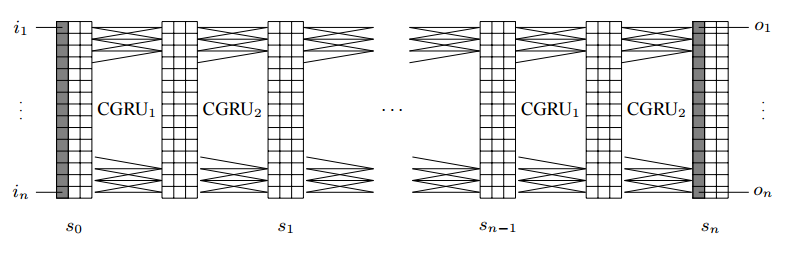
\includegraphics[scale=0.5]{Imgs/NeuralGPU.png}
	\caption{معماری ارائه شده در پژوهش حاضر}
	\label{fig:arch}
\end{figure}


\section{جمع‌بندی}
در این فصل از گزارش، چارچوب کاری رمزگذار-رمزگشا را در حالت استاندارد مورد بررسی قرار دادیم. در این چارچوبِ، معمولا از یک شبکه عصبی کانولوشنی عمیق به عنوان رمزگذار استفاده می‌شود. بسته به این که در فرایند پژوهش، توجه بصری مورد استفاده قرار گرفته یا خیر، رمزگذار می‌تواند یک یا بیش از یک بردار ویژگی از تصویر استخراج نماید.
\\
در این پژوهش از شبکه عصبی \lr{Google Inception V3} به عنوان رمز‌گذار استفاده شده است. این شبکه کانولوشنی، برای دسته‌بندی تصاویر موجود در مجموعه‌داده \lr{ImageNet} مورد آموزش قرار گرفته است و در حال حاضر به صورت از پیش آموزش دیده، در دسترس پژوهش‌گران می‌باشد. برای استفاده از این شبکه عصبی در کاربرد تولید خودکار شرح بر تصایر، لازم است، به جای خروجی لایه آخر شبکه، از خروجی دومین لایه قبل از لایه آخر به عنوان خروجی رمزگذار استفاده شود.
\\
خروجی دومین لایه قبل از لایه آخر در این شبکه، به لایه انتقال یادگیری معروف است. زیرا این لایه، تمام اطلاعات استخراج شده از تصویر را در خود نگه‌داری می‌کند و دو لایه آخر این شبکه که لایه‌های تماما متصل هستند، به منظور استفاده از این شبکه در حوزه دسته‌بندی تصاویر مورد آموزش قرار گرفته‌اند و در کاربرد تولید خودکار شرح بر تصاویر، قابل استفاده نیستند. 
\\
لایه انتقال یادگیری در این شبکه کانولوشنی شامل تعداد $8*8$ بردار 2048 بعدی است که هر یک از این بردارها، علاوه بر این‌که اطلاعات استخراج شده از کل تصویر را در خود نگه‌داری می‌کنند، بر روی بخشی از تصویر ورودی تمرکز دارند. این بردارها می‌توانند به عنوان بردارهای حاشیه‌نویسی تصویر مورد استفاده قرار بگیرند.
\\
در حال حاضر، طراحی و حل معضلات موجود در بخش رمزگشا در این چارچوب کاری، چالش‌ برانگیزتر از بخش رمزگذار به حساب می‌آید. وظیفه رمزگشا این است که با دریافت بردار یا بردارهای ویژگی تصویر که توسط رمزگذار استخراج شده است، شرح توصیف‌کننده تصویر را به صورت کلمه به کلمه تولید نماید. 
\\
در این پژوهش، از شبکه \lstm به عنوان واحد اصلی شبکه بازگشتی استفاده شده است. روابط \eqref{eq:lstm1} تا \eqref{eq:lstm5}، ساختار یک واحد \lstm را مدل‌سازی می‌نمایند. همین‌طور شکل \ref{fig:lstm}، طرح‌واره‌ای از یک واحد \lstm را نمایش می‌دهد. چینش این واحد‌ها به صورت پشته‌ای بر روی هم، یک لایه از شبکه رمزگشا را تشکیل می‌دهد که در هر واحد زمانی، یک کلمه را تولید می‌نماید. شکل \ref{fig:stackedLstm}، ساختار پشته‌ای شبکه رمزگشا را نمایش می‌دهد.
\\
در تمامی پژوهش‌های انجام شده در این حوزه، این تولید کلمه به کلمه را به صورت پیش‌بینی احتمال شرطی کلمه بعدی به شرط داشتن کلمات تولید‌شده قبلی و بردار یا بردارهای ویژگی تصویر، مدل می‌نمایند.
\\
در این حالت، بردار خروجی شبکه در هر مرحله باید به تعداد کلمات موجود در دیکشنری کلمات، مولفه داشته باشد و هر مولفه از این بردار، احتمال رخداد کلمه متناظر خود در دیکشنری کلمات را نمایش دهد. برای تضمین این نکته که خروجی شبکه در هر مرحله حتما یک توزیع احتمال خواهد بود، یک لایه \lr{Soft Max} به انتهای شبکه اضافه می‌شود تا خروجی تولید شده را به یک توزیع احتمال تبدیل نماید.
\\
با توجه به این نکته که شبکه در هر مرحله باید یک توزیع احتمال روی کلمات تولید نماید، در مرحله آموزش شبکه، کلمات موجود در شرح متناظر تصاویر در مجموعه‌داده آموزشی، باید به صورت بردار تک‌فعال درآمده و به عنوان مقدار مطلوب هر مرحله به شبکه داده شوند. به عبارت بهتر، مقدار مطلوب برای توزیع احتمال مطلوب شبکه در مرحله $t$ام از تولید جمله، یک بردار به طول تعداد کلمات موجود در دیکشنری است که تمام مولفه‌های آن مقدار صفر دارند و فقط مولفه‌ای از این بردار که اندیس آن با اندیس کلمه $t+1$ام در شرح موجود برای تصویر در دیکشنری لغات برابر است، مقدار یک دارد.
\\
استفاده از بردار تک‌فعال به عنوان خروجی مطلوب شبکه، باعث ایجاد مشکلاتی می‌شود که از جمله آن‌ها می‌توان به نکات زیر اشاره کرد:
\begin{enumerate}
	\item عدم استفاده از اطلاعات معنایی کلمات، استفاده از کلمات مترادف و تولید جملات متنوع‌تر
	\item تنک‌شدن مقدار مطلوب شبکه و کاهش قدرت شبکه در یادگیری پارامترها
	\item افزایش چشم‌گیر تعداد پارامترهای قابل یادگیری شبکه به دلیل بالابودن ابعاد خروجی در تمام مراحل
\end{enumerate}

روش پیشنهادی در این پژوهش، به منظور حل مشکلات فوق‌الذکر، استفاده از بردار جاسازی کلمات به جای بردار تک‌فعال به عنوان بردار مطلوب شبکه است. این جایگزینی علاوه بر ایجاد امکان استفاده از اطلاعات معنایی کلمات، از تنک شدن مقادیر مطلوب شبکه جلوگیری می‌نماید. همین‌طور استفاده از جاسازی کلمات، امکان کاهش چشم‌گیر اندازه خروجی مطلوب شبکه در هر مرحله را فراهم نموده و پیرو آن باعث کاهش دادن اندازه شبکه شده، تعداد پارامترهای قابل آموزش را کاهش داده و روند یادگیری شبکه را سهولت می‌بخشد.
\\
به منظور ایجاد جاسازی مناسب برای کلمات، از مدل \lr{Skip-Gram} ارائه شده در پژوهش \cite{mikolov2013distributed} استفاده شده است. در این مدل، مطابق با رابطه \eqref{eq:embd}، جاسازی کلمات به نحوی تولید می‌شود که با داشتن بردار جاسازی یک کلمه، بتوان بردارهای جاسازی کلمات قبل و بعد را دسته‌بندی نمود. این خاصیت در بردارهای جاسازی مورد استفاده، علاوه بر حل مشکلات بردار تک‌فعال، باعث سهولت بیشتر شبکه بازگشتی در تولید بردارهای جاسازی بعدی می‌شود.
\\
لازم به توضیح است، جاسازی تمام کلمات موجود در دیکشنری، در این پژوهش با استفاده از جملات موجود در توصیفات تصاویر مجموعه‌داده آموزشی، انجام شده است. به عبارت بهتر، مدل جاسازی کلمات، با دریافت تمام توصیفات موجود در مجموعه‌داده آموزشی، برای تمام کلمات موجود در دیکشنری، بردار جاسازی متناظر را تولید می‌نماید و در تمام فرایندهای بعدی، شامل فرایند‌های آموزش و تست شبکه، از این بردارهای جاسازی از پیش ذخیره شده، مستقیما استفاده می‌شود.
\\
با تغییر خروجی مطلوب شبکه از حالت بردار تک‌فعال به بردار جاسازی، مساله \eqref{eq:obj1}، که یک مساله پیش‌بینی توزیع احتمال است، به مساله \eqref{eq:obj2}، که یک مساله رگرسیون به حساب می‌آید، تغییر پیدا می‌کند. برای حل این مساله رگرسیون، ناگزیر به تغییر تابع خطای شبکه از تابع هزینه \lr{Cross Entropy} به تابع میانگین مربع خطا هستیم.
\\
در فرایند آموزش شبکه، از بهینه‌ساز آدام استفاده شده است. به علاوه برای جلوگیری از بیش‌برازش شبکه بازگشتی روی داده‌های موجود در مجموعه‌داده آموزشی، از منظم‌ساز حذف نود که یکی از پرکاربردترین منظم‌ساز‌های مورد استفاده در پژوهش‌های حوزه تولید خودکار شرح بر تصاویر به شمار می‌رود، استفاده شده است.



